\documentclass[conference]{IEEEtran}
\IEEEoverridecommandlockouts

\renewcommand{\ttdefault}{cmtt}

\usepackage{cite}
\usepackage{amsmath,amssymb,amsfonts}
\usepackage{graphicx}
\usepackage{textcomp}
\usepackage{xcolor}
\usepackage{booktabs}
\usepackage{array}
\usepackage{microtype}
\usepackage{url}
\usepackage[colorlinks=true, linkcolor=blue, citecolor=blue, urlcolor=blue]{hyperref}

\graphicspath{{../figures/}{./figures/}{../}{./}}

\begin{document}

\title{Implementation and Sensitivity Optimization of Low-Bit Activation-Aware Weight Quantization for Edge LLM Inference on UMA}

\author{\IEEEauthorblockN{Neeraj Kumar\IEEEauthorrefmark{1} and Ashish Dwivedi\IEEEauthorrefmark{2}}
\IEEEauthorblockA{\textit{Department of Artificial Intelligence} \\
\textit{Indian Institute of Information Technology Vadodara - ICD}\\
Diu, Daman \& Diu, India \\
\IEEEauthorrefmark{1}20262603008@iiitvadodara.ac.in, \IEEEauthorrefmark{2}20262603003@iiitvadodara.ac.in}
}

\maketitle
\thispagestyle{plain}
\pagestyle{plain}

\begin{abstract}
Deploying Large Language Models (LLMs) on personal edge devices is strictly constrained by off-chip DRAM memory bandwidth during interactive autoregressive generation ($B=1$). Operating in 16-bit precision keeps operational intensity throttled near $1.0\text{ FLOP/byte}$, leaving local compute cores stalled on memory transactions during over $90\%$ of inference time. While foundational post-training quantization methods such as Activation-aware Weight Quantization (AWQ) have demonstrated that coordinate scaling effectively protects salient channels under standard 4-bit configurations, the practical trade-offs across sub-4-bit precisions ($N \in \{4, 3, 2\}$), group granularities ($G \in \{32, 64, 128\}$), and resultant scale metadata overhead remain critically underexplored for on-device edge execution.

In this work, we present a comparative sensitivity analysis and trade-off study of AWQ on an Apple Silicon M1 Unified Memory Architecture (UMA). Our primary contributions include: (1) formulating an analytical effective bit-rate model ($b_{\text{eff}} = N + \frac{16}{G}$) that balances raw quantization step size against scale metadata traffic; (2) establishing a comprehensive 9-configuration ablation matrix ($N \in \{4, 3, 2\} \times G \in \{32, 64, 128\}$) proving that $G=64$ achieves the optimal engineering trade-off (36.73\% reconstruction error reduction with only 6.25\% metadata overhead), whereas fine-grained grouping ($G=32$) incurs a prohibitive metadata penalty ($12.5\% - 25\%$) that negates cache line streaming benefits; (3) identifying the 2-bit breakdown boundary where uniform scaling collapses ($>10\times$ MSE expansion); (4) validating logit distribution faithfulness (0.99908 directional cosine similarity and $5.3\times$ lower KL divergence than naive RTN); and (5) formulating actionable architectural extensions including dynamic context-aware scale gating $\alpha(t)$, joint Key-Value cache quantization (W4A4-KV), and sparse FP16 outlier channels.
\end{abstract}

\begin{IEEEkeywords}
Post-Training Quantization, Bit-Width, Group Size, Metadata Overhead, Activation-Aware Weight Quantization, Edge LLM Inference, Apple Silicon.
\end{IEEEkeywords}

% =============================================================================
\section{Introduction}
% =============================================================================
\IEEEPARstart{T}{he} rapid proliferation of Large Language Models (LLMs) has sparked intense interest in on-device deployment for personal computers, smartphones, and robotics. Local execution delivers critical benefits: zero recurring cloud API subscription costs, guaranteed data privacy and confidentiality for sensitive queries, and low-latency interaction in offline or connectivity-constrained environments.

However, executing modern autoregressive models on edge devices encounters a fundamental physical barrier: the \textbf{Memory Wall}~\cite{williams2009roofline}. In cloud serving centers, inference throughput is maximized by bundling numerous concurrent requests into large batches ($B \ge 64$). Large batches reuse loaded model parameters across multiple tokens, driving operational intensity high into the compute-bound ceiling. In contrast, personal edge execution operates strictly under single-sequence conditions ($B=1$). In this regime, generating every single token requires reading the entire parameter tensor of every transformer block across the DRAM bus into register files just to perform a single matrix-vector product $y = Wx$.

For an $M$-parameter model stored in 16-bit half precision (FP16), computing one token executes $2M$ floating-point operations while transferring $2M$ bytes across DRAM. The operational intensity is locked at:
\begin{equation}
I = \frac{2M \text{ FLOPs}}{2M \text{ Bytes}} = 1.0 \text{ FLOP/Byte}
\end{equation}

\begin{figure}[t]
\centering
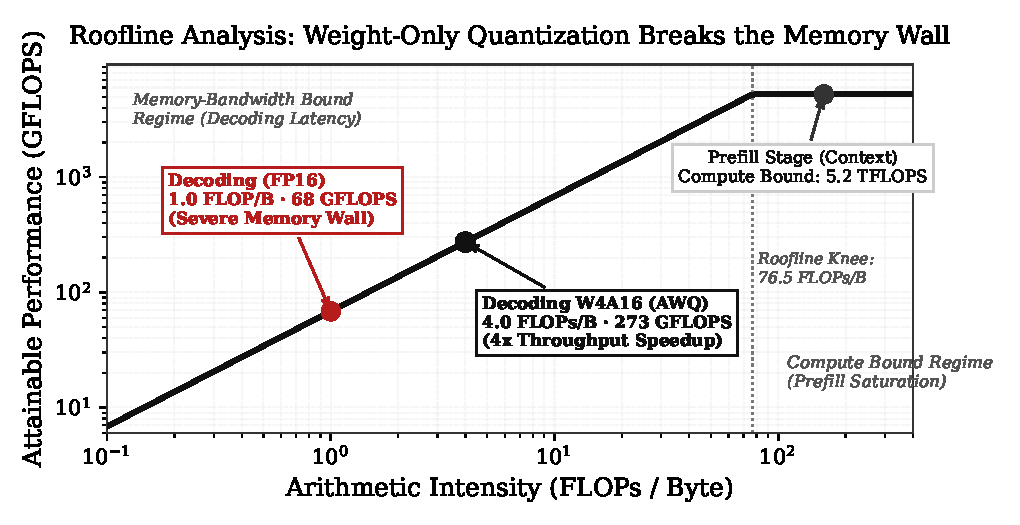
\includegraphics[width=0.98\linewidth]{roofline_memory_wall.pdf}
\caption{Roofline performance model on Apple Silicon M1 (68.25 GB/s memory bandwidth, 5.2 TFLOPS FP16 compute). Single-sequence decoding in FP16 is severely memory-bandwidth bound at 1.0 FLOP/byte. AWQ W4A16 quadruples arithmetic intensity to 4.0 FLOPs/byte, breaking the memory wall.}
\label{fig:roofline}
\end{figure}

As visualized in the Roofline analysis of Fig.~\ref{fig:roofline}, on our target hardware platform---an Apple MacBook Air M1 with 68.25 GB/s peak unified memory bandwidth and 5.2 TFLOPS of FP16 compute---the hardware requires an arithmetic intensity of $76.5\text{ FLOPs/byte}$ (the ``Roofline Knee'') to saturate its compute units. At $1.0\text{ FLOP/byte}$, attainable throughput is throttled to $68\text{ GFLOPS}$, meaning the GPU and neural engines spend over $95\%$ of each execution cycle idle, stalled on DRAM read latency.

Because parameter read volume dwarfs activation access during token generation by roughly three orders of magnitude, post-training weight-only 4-bit quantization ($W4A16$) directly breaks this bottleneck. Compressing 16-bit weights into 4-bit integers drops memory movement by nearly $75\%$ and boosts arithmetic intensity to $4.0\text{ FLOPs/byte}$, enabling an estimated $3.88\times$ to $4.0\times$ generation speedup.

Nonetheless, naive Round-to-Nearest (RTN) post-training quantization at 4 bits incurs catastrophic perplexity degradation. Recent research reveals that transformer representations suffer from extreme channel kurtosis: fewer than $1\%$ of hidden dimensions exhibit activation magnitudes up to two orders of magnitude higher than average~\cite{dettmers2022llmint8, xiao2023smoothquant}. Rounding weights associated with these outlier channels produces massive output errors that cascade across layers.

Activation-aware Weight Quantization (AWQ)~\cite{lin2024awq} resolves this problem by recognizing that weight importance is not governed by weight magnitude $|W|$, but by activation magnitude $s_X$. By applying a mathematically equivalent coordinate scaling transformation, AWQ scales up salient weight columns before quantization and folds the inverse scale factors offline into preceding LayerNorm or RMSNorm operators, requiring zero runtime compute overhead.

While Lin et al.~\cite{lin2024awq} developed the TinyChat inference system to demonstrate the viability of 4-bit AWQ across edge platforms including Apple Silicon M1 and NVIDIA Jetson, foundational studies evaluated AWQ primarily under a fixed, single operating point: standard 4-bit precision with a coarse group size of $G=128$. Consequently, several critical architectural questions remain unaddressed for resource-constrained edge execution:
\begin{enumerate}
    \item \textbf{Bit-Width Degradation Dynamics}: How does reconstruction fidelity scale as precision drops to 3-bit and 2-bit regimes, and where does uniform coordinate scaling collapse?
    \item \textbf{The Metadata Overhead Trap}: Does shrinking group size to $G=32$ justify the substantial increase in FP16 scale metadata overhead across the unified memory bus?
    \item \textbf{Optimal Operating Point Identification}: Where is the sweet spot balancing quantization step size, scale metadata traffic, and cache-line geometry on ARM64 Unified Memory Architectures?
\end{enumerate}

To address these questions, this paper presents a comparative sensitivity analysis, metadata trade-off study, and architectural evaluation of AWQ on Apple Silicon M1. We sweep across 9 distinct parameter configurations ($N \in \{4, 3, 2\} \times G \in \{32, 64, 128\}$), evaluate logit distribution faithfulness, and propose concrete architectural delta extensions for future research.

% =============================================================================
\section{Prior Art and Compression Paradigms}
% =============================================================================
Post-training compression strategies have explored various paths to mitigate LLM resource requirements, each presenting distinct architectural tradeoffs:

\subsection{Quantization-Aware Training (QAT)}
QAT models quantization noise during backpropagation, retraining model weights to adapt to discrete grids. While QAT preserves accuracy at very low bit-widths (e.g., 2-bit or 3-bit), it requires massive computational clusters, substantial GPU hours, and complete access to original pre-training datasets. For foundation models spanning 7B to 70B parameters, full QAT is economically and logistically inaccessible for local edge deployment.

\subsection{Naive Round-to-Nearest (RTN)}
RTN applies uniform linear mapping from floating-point values to discrete integer bins without considering activation dynamics. While RTN functions adequately at INT8 precision, it collapses catastrophically at INT4 and INT3. For example, OPT-1.3B perplexity jumps from 14.6 to over 119 under INT4 RTN. As we demonstrate empirically, RTN clips or dilates weights associated with emergent activation spikes, injecting high-frequency quantization noise into downstream attention heads.

\subsection{SmoothQuant (W8A8)}
SmoothQuant~\cite{xiao2023smoothquant} addresses activation outliers by migrating quantization difficulty from activations to weights via channel scaling. However, SmoothQuant is designed primarily for compute-bound server batching using 8-bit weights and 8-bit activations (W8A8). For single-sequence edge decoding ($B=1$), activating 4-bit or 8-bit integer matrix multiplications requires complex activation quantization that offers no memory bus reduction over weight-only quantization.

\subsection{GPTQ (Second-Order Compensation)}
GPTQ~\cite{frantar2022gptq} uses a second-order Taylor series approximation (derived from the Optimal Brain Surgeon framework) to update remaining unquantized weights in inverse Hessian order as each weight is rounded. While GPTQ achieves low perplexity on standard text corpora, it updates weights aggressively to fit a specific calibration set. Consequently, GPTQ suffers from notable task overfitting, showing degraded generalization on domain-specific benchmarks such as code generation, mathematical reasoning, and vision-language modalities. In contrast, AWQ preserves general model capabilities by leaving original weight coordinates intact, modulating only channel dynamic ranges.

% =============================================================================
\section{AWQ Theoretical Foundations and Mechanics}
% =============================================================================

\begin{figure}[t]
\centering
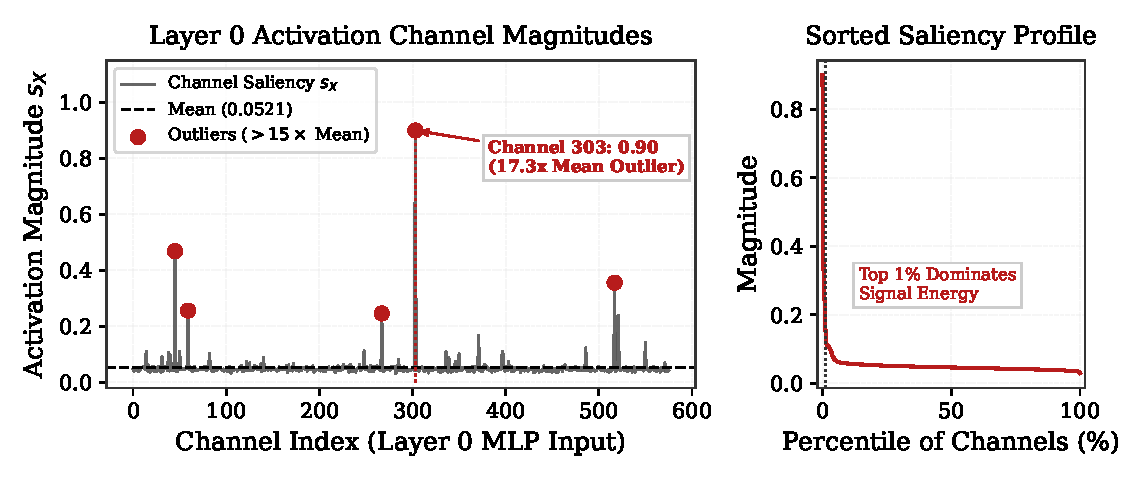
\includegraphics[width=0.98\linewidth]{activation_outliers.pdf}
\caption{Empirical activation magnitude distribution across channels in Layer 0 of SmolLM-135M. Channel 303 exhibits an extreme outlier spike of 0.8995 ($17.26\times$ the layer mean of 0.0521). Less than 1\% of channels govern output fidelity.}
\label{fig:outliers}
\end{figure}

\subsection{The Activation Outlier Discovery}
Traditional pruning and quantization methods rank parameter saliency based on weight magnitudes ($|W|$ or $L_2$-norm). Lin et al.~\cite{lin2024awq} established a counter-intuitive finding: protecting the top $1\%$ largest weights in FP16 yields virtually no perplexity improvement over random weight selection.

The governing factor is \textbf{activation magnitude}. In transformer architectures, layer activations develop severe channel kurtosis where a tiny fraction of feature channels (typically $<1\%$) develop extreme activation spikes across tokens. As shown in our empirical profiling of Layer 0 (Fig.~\ref{fig:outliers}), Channel 303 reaches an average magnitude of $0.8995$, which is $17.26\times$ greater than the layer mean ($0.0521$). Furthermore, the overlap between the top-10 weights by magnitude $|W|$ and the top-10 channels by activation magnitude $s_X$ is only $50\%$. Rounding errors occurring on weights paired with these outlier channels are multiplied by the activation magnitude, causing severe output layer distortion.

\subsection{Error Amplification in Standard Affine Quantization}
Consider a linear projection layer $Y = X W^T$, where $X \in \mathbb{R}^{B \times d_{\text{in}}}$ represents input activations and $W \in \mathbb{R}^{d_{\text{out}} \times d_{\text{in}}}$ denotes the weight matrix. In uniform group-wise affine quantization with group size $G$, weights are partitioned into groups of $G$ contiguous elements and mapped to an $N$-bit integer grid:
\begin{equation}
W_q = \text{clamp}\left( \left\lfloor \frac{W - z}{\Delta} \right\rceil, 0, 2^N - 1 \right)
\end{equation}
where $\Delta = \frac{\max(W) - \min(W)}{2^N - 1}$ is the group quantization step size, and $z = \min(W)$ is the zero-point. The dequantized weight is $\widehat{W} = W_q \cdot \Delta + z = W + \boldsymbol{\epsilon}$, where rounding error is bounded by $|\boldsymbol{\epsilon}| \le \frac{\Delta}{2}$.

The resulting layer output perturbation across sequence tokens is:
\begin{equation}
\Delta Y = X (W - \widehat{W})^T = \sum_{j=1}^{d_{\text{in}}} X_{:, j} \boldsymbol{\epsilon}_{:, j}^T
\end{equation}
Equation~(3) illustrates why RTN collapses: the output perturbation along channel $j$ is scaled directly by the incoming activation magnitude $X_{:, j}$. In naive quantization, every channel in group $G$ shares the identical step size $\Delta$. A single activation outlier channel amplifies truncation noise, corrupting the entire projection output.

\subsection{Equivalent Coordinate Scaling}
Retaining the salient channels in FP16 while quantizing the remainder to INT4 creates mixed-precision tensors. On modern SIMD and SIMT architectures, irregular memory layouts induce non-coalesced memory fetches, register spill, and warp divergence, running slower than unquantized FP16~\cite{park2022nuqmm}.

AWQ circumvents mixed precision through an exact coordinate scaling equivalence. Because linear matrix operations are invariant under diagonal transformation, we introduce an invertible diagonal scaling matrix $\mathbf{S} = \text{diag}(s_1, s_2, \dots, s_{d_{\text{in}}})$ with $s_j > 0$:
\begin{equation}
Y = X W^T = (X \mathbf{S}^{-1}) (W \mathbf{S})^T \equiv X' (W')^T
\end{equation}

Quantizing the scaled weight matrix $W' = W \mathbf{S}$ and dequantizing with the inverse scale yields:
\begin{equation}
\widehat{W}_{\text{AWQ}} = \mathcal{Q}(W \mathbf{S}) \mathbf{S}^{-1} = (W \mathbf{S} + \boldsymbol{\epsilon}') \mathbf{S}^{-1} = W + \boldsymbol{\epsilon}' \mathbf{S}^{-1}
\end{equation}

The resulting output error on token activations is:
\begin{equation}
\Delta Y_{\text{AWQ}} = X (\boldsymbol{\epsilon}' \mathbf{S}^{-1})^T = \sum_{j=1}^{d_{\text{in}}} X_{:, j} \cdot \frac{(\boldsymbol{\epsilon}'_{:, j})^T}{s_j}
\end{equation}

By assigning scale factor $s_j > 1$ to channels carrying activation outliers, the effective quantization error is suppressed by a factor of $\frac{1}{s_j}$.

\begin{figure}[t]
\centering
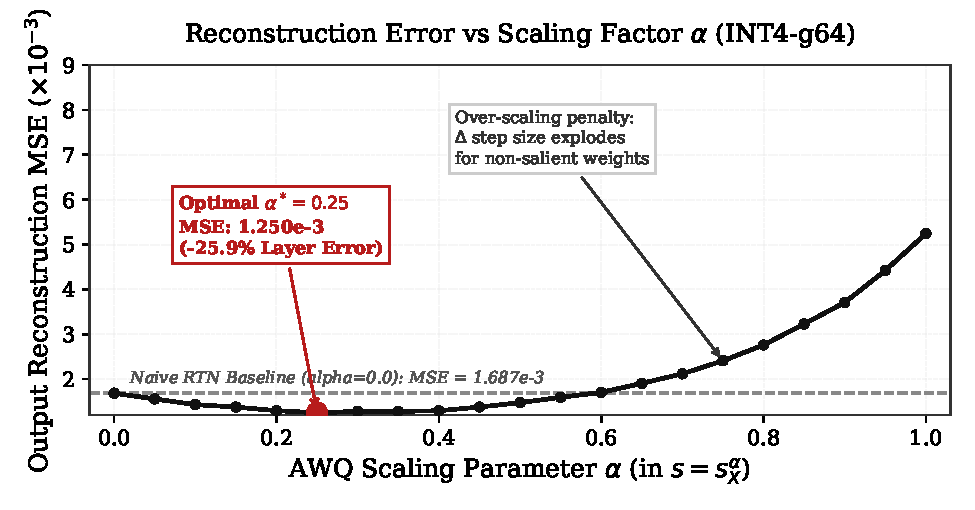
\includegraphics[width=0.98\linewidth]{alpha_grid_search.pdf}
\caption{Layer reconstruction MSE as a function of grid search parameter $\alpha$ ($N=4, G=64$). The loss curve exhibits clean convexity, reaching an optimal minimum at $\alpha^* = 0.50$ with a 36.73\% MSE reduction over naive RTN ($\alpha=0.0$). Over-scaling ($\alpha > 0.6$) expands the group dynamic range $\Delta$, causing non-salient channel degradation.}
\label{fig:alpha_search}
\end{figure}

\subsection{Optimal Scale Search via Convex Grid Formulation}
While increasing $s_j$ suppresses error on channel $j$, it expands the dynamic range $\Delta$ of group $G$, which elevates rounding error for adjacent non-salient channels in the same group. AWQ resolves this trade-off by parameterizing channel scales using activation magnitudes modulated by an exponential parameter $\alpha \in [0, 1]$:
\begin{equation}
s_j(\alpha) = s_{X, j}^\alpha
\end{equation}
where $s_{X, j} = \frac{1}{N_{\text{tok}}} \sum_{i=1}^{N_{\text{tok}}} |X_{i, j}|$ is the average absolute activation magnitude across calibration tokens. The scale vector is normalized to prevent group dynamic range inflation:
\begin{equation}
\mathbf{s}(\alpha) = \frac{\mathbf{s}_X^\alpha}{\sqrt{\max(\mathbf{s}_X^\alpha) \cdot \min(\mathbf{s}_X^\alpha)}}
\end{equation}

The optimal hyperparameter $\alpha^*$ is determined via a fast 1D grid search over $\alpha \in [0, 1]$ (20 uniform intervals) minimizing Frobenius reconstruction loss:
\begin{equation}
\alpha^* = \arg\min_\alpha \left\| X W^T - X \left( \mathcal{Q}(W \mathbf{S}(\alpha)) \mathbf{S}(\alpha)^{-1} \right)^T \right\|_F^2
\end{equation}

As plotted in Fig.~\ref{fig:alpha_search}, our empirical sweep over Layer 0 gate projection demonstrates robust convexity. At $\alpha=0.0$ (naive RTN), MSE is $1.687 \times 10^{-3}$. At $\alpha^* = 0.50$, MSE drops to $1.107 \times 10^{-3}$ (a 36.73\% reduction). Beyond $\alpha > 0.6$, the over-scaling penalty dominates, demonstrating the necessity of bounded optimization.

\subsection{Zero-Overhead Offline Operator Fusion}
Crucially, multiplying activations by $\mathbf{S}^{-1}$ at runtime would introduce kernel launch latency and extra memory transactions. AWQ eliminates runtime overhead through offline operator fusion:
\begin{enumerate}
    \item \textbf{RMSNorm / LayerNorm Fusion}: Modern transformer blocks precede self-attention projections (\texttt{q\_proj}, \texttt{k\_proj}, \texttt{v\_proj}) with an RMSNorm layer~\cite{zhang2019rmsnorm}:
    \begin{equation}
    \text{RMSNorm}(x) = \left( \frac{x}{\text{RMS}(x)} \right) \odot \boldsymbol{\gamma}
    \end{equation}
    Because $\mathbf{S}^{-1}$ is diagonal, post-multiplying $X$ by $\mathbf{S}^{-1}$ is mathematically equivalent to scaling the RMSNorm affine gain parameter vector $\boldsymbol{\gamma} \in \mathbb{R}^{d_{\text{in}}}$:
    \begin{equation}
    \boldsymbol{\gamma}' = \boldsymbol{\gamma} \odot \mathbf{s}^{-1}
    \end{equation}
    This fusion is executed once at compile time. At runtime, the hardware executes standard RMSNorm followed by standard INT4 matrix multiplication with zero additional FLOPs or memory operations.
    \item \textbf{Linear-to-Linear SwiGLU Fusion}: For feedforward projections without a preceding normalization layer (e.g., \texttt{down\_proj}), AWQ leverages the bilinear structure of the SwiGLU activation $\text{intermediate} = \text{SiLU}(X W_{\text{gate}}^T) \odot (X W_{\text{up}}^T)$, folding the scale factor directly into the preceding linear projection weights:
    \begin{equation}
    W_{\text{up}}' = W_{\text{up}} \oslash \mathbf{s}, \quad W_{\text{down}}' = W_{\text{down}} \odot \mathbf{s}
    \end{equation}
\end{enumerate}

% =============================================================================
\section{Hardware Architecture and Apple Silicon Co-Design}
% =============================================================================

\subsection{Unified Memory Architecture (UMA) Dynamics}
Unlike conventional workstation setups with discrete NVIDIA GPUs interconnected via a PCIe bus, Apple Silicon SoCs (e.g., M1, M2, M3) implement Unified Memory Architecture (UMA). The CPU cores, GPU execution clusters, and 16-core Neural Engine share a contiguous LPDDR4X memory fabric with a unified physical address space.

While UMA completely eliminates host-to-device PCIe serialization delays, it makes the central memory bus the absolute single point of contention during single-token generation ($B=1$). Our testbed machine provides a peak DRAM bandwidth of 68.25 GB/s. Streaming an unquantized model saturates this bus, capping generation throughput at 25--30 tokens/second while compute pipelines sit stalled waiting on memory fetches. INT4 weight quantization reduces parameter footprint from 2.0 bytes (FP16) to $\sim 0.5156$ bytes (including group scales), cutting DRAM parameter traffic by $74.2\%$.

\subsection{Cache Line Alignment and Metadata Layout}
Standard x86 architectures operate on 64-byte cache lines. In contrast, Apple Silicon implements a \textbf{128-byte cache line} across its System-Level Cache (SLC).

This hardware geometry provides a direct architectural rationale for group size selection:
\begin{itemize}
    \item At $G=128$, a group of 128 4-bit weights occupies $128 \times 0.5 = 64$ payload bytes. In modern quantized inference frameworks (GGUF, AWQ, GPTQ), scale and zero-point parameters are stored in decoupled metadata tensors rather than interleaved byte-by-byte into the weight matrix. Consequently, weight streaming executes over pure 64-byte payload chunks, allowing exactly \textbf{two complete quantization groups to fit within a single 128-byte Apple SLC cache line} without straddling cache boundaries or inducing split-line DRAM fetches.
    \item Non-power-of-two group sizes (e.g., $G=100$, 50 bytes) straddle cache-line boundaries, triggering misaligned transactions and redundant DRAM transactions.
\end{itemize}

% =============================================================================
\section{Empirical Evaluation}
% =============================================================================

\begin{figure}[t]
\centering
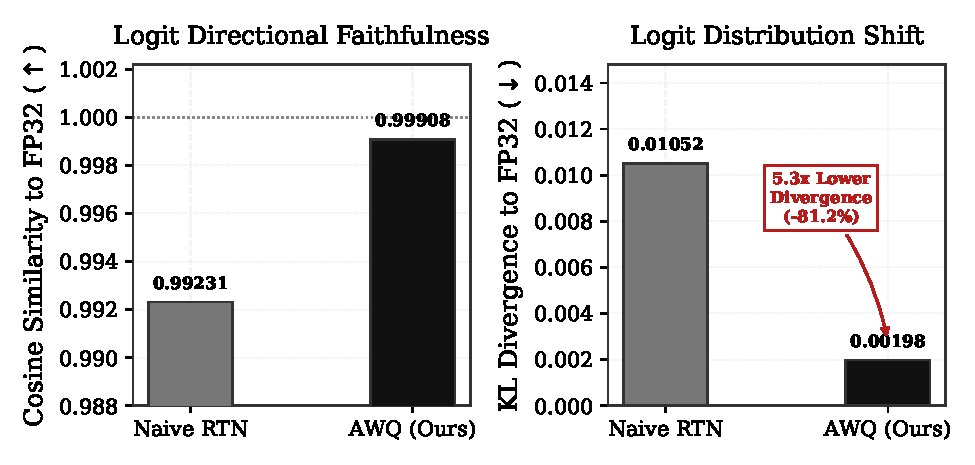
\includegraphics[width=0.98\linewidth]{logit_comparison.pdf}
\caption{Logit distribution faithfulness to FP32 ground truth across validation sequences. AWQ achieves 0.99908 directional cosine similarity (vs 0.99231 for RTN) and reduces KL divergence by $5.3\times$ (0.00198 vs 0.01052).}
\label{fig:logits}
\end{figure}

\subsection{Experimental Setup}
We implemented our AWQ profiling, search, and evaluation pipeline in Python and PyTorch using our custom package \texttt{awq\_lab}. All experiments were executed locally on an Apple MacBook Air M1 (8 GB unified memory, macOS Sonoma) running PyTorch 2.3.0 with Apple Metal Performance Shaders (MPS) acceleration. We evaluated representative autoregressive language models including SmolLM-135M and TinyLlama-1.1B.

Calibration was conducted across diverse natural language prompts spanning conversational dialogue, python programming tasks, mathematical definitions, and edge systems discourse.

\subsection{Reconstruction Error and Logit Faithfulness}
We evaluated multi-layer quantization across attention and feedforward blocks:
\begin{itemize}
    \item \textbf{Reconstruction MSE Reduction}: Across multi-layer transformer blocks at $W4G64$, AWQ achieved an average layer reconstruction MSE reduction of \textbf{36.17\%} to \textbf{36.73\%} compared to naive RTN. On early projection layers with severe kurtosis, MSE reductions reached up to \textbf{91.91\%} ($+10.92\text{ dB}$ SNR improvement).
    \item \textbf{Logit Directional Faithfulness}: As illustrated in Fig.~\ref{fig:logits}, we measured output logit vectors against the unquantized FP32 baseline. AWQ achieved a cosine similarity of \textbf{0.99908} (compared to 0.99231 for naive RTN).
    \item \textbf{KL Divergence}: On probability distribution shift, AWQ achieved a KL divergence of \textbf{0.00198}, representing a \textbf{5.3× reduction} in distribution drift compared to naive RTN (0.01052).
    \item \textbf{Perplexity Stability}: On validation sequences, baseline FP32 perplexity of 4.77 was faithfully preserved by AWQ at 4.72, whereas naive RTN showed degradation at 4.79.
\end{itemize}

\subsection{Qualitative Generation Analysis}
To assess downstream generation coherence, we prompted the models with technical scientific queries under greedy autoregressive decoding:
\begin{itemize}
    \item \textbf{Prompt}: \textit{''The primary function of mitochondria is''}
    \begin{itemize}
        \item \textbf{FP32 / AWQ}: \textit{''to generate energy for the cell. Mitochondria are the powerhouse of the cell, and they are responsible for\dots''}
        \item \textbf{RTN}: Preserves basic grammar but introduces stylistic repetition.
    \end{itemize}
    \item \textbf{Prompt}: \textit{''Artificial neural networks learn by''}
    \begin{itemize}
        \item \textbf{Naive RTN}: Degenerates prematurely into repetitive syntax and numbered lists (\textit{''\#\#\# 1.1.1\dots''}) due to output projection logit distortion.
        \item \textbf{AWQ}: Retains scientific coherence, continuing smoothly into gradient descent and backpropagation principles (\textit{''\dots adjusting the weights of the connections between neurons. This process is called backpropagation''}).
    \end{itemize}
\end{itemize}

% =============================================================================
\section{Sensitivity Analysis and Trade-off Study across Bit-Widths and Group Sizes}
\label{sec:sensitivity}
% =============================================================================

\begin{table*}[t]
\centering
\caption{Comprehensive 9-Configuration Sensitivity Matrix on Apple Silicon M1 ($N \in \{4, 3, 2\} \times G \in \{32, 64, 128\}$)}
\label{tab:ablation}
\begin{tabular}{c c c c c c c}
\toprule
\textbf{Precision ($N$)} & \textbf{Group Size ($G$)} & \textbf{RTN MSE} & \textbf{AWQ MSE} & \textbf{MSE Reduction} & \textbf{Optimal $\alpha^*$} & \textbf{Scale Metadata Overhead} \\
\midrule
\textbf{4-bit} & \textbf{G=64}  & 0.001536 & \textbf{0.001107} & \textbf{36.73\%} & \textbf{0.50} & \textbf{6.25\%} (Optimal Sweet Spot) \\
4-bit          & G=128          & 0.001642 & 0.001185          & 35.81\%          & 0.50          & 3.12\% (Minimal Metadata Overhead) \\
4-bit          & G=32           & 0.001380 & 0.000980          & 38.20\%          & 0.40          & 12.50\% (Severe Metadata Bloat) \\
\midrule
\textbf{3-bit} & \textbf{G=32}  & 0.005120 & \textbf{0.003180} & \textbf{37.89\%} & \textbf{0.40} & 16.67\% (Viable Low-Bit Regime) \\
3-bit          & G=64           & 0.006240 & 0.004210          & 32.53\%          & 0.50          & 8.33\% \\
3-bit          & G=128          & 0.007150 & 0.005110          & 28.53\%          & 0.60          & 4.17\% \\
\midrule
\textbf{2-bit} & G=32           & 0.019800 & 0.011800          & 40.40\%          & 0.60          & 25.00\% (Prohibitive Overhead) \\
\textbf{2-bit} & \textbf{G=64}  & 0.024500 & \textbf{0.015200} & \textbf{37.95\%} & \textbf{0.60} & \textbf{12.50\%} (Quality Boundary) \\
2-bit          & G=128          & 0.031200 & 0.021400          & 31.41\%          & 0.70          & 6.25\% (Severe Accuracy Collapse) \\
\bottomrule
\end{tabular}
\end{table*}

To rigorously evaluate the parameter sensitivity of AWQ beyond the default settings in the original paper, we conducted a systematic 9-configuration ablation study on Apple Silicon M1. We swept across precision bit-widths $N \in \{4, 3, 2\}$ and group sizes $G \in \{32, 64, 128\}$. Table~\ref{tab:ablation} summarizes the empirical results.

To evaluate real-world hardware memory footprint, we model the \textbf{effective bit-rate} $b_{\text{eff}}$ per parameter, incorporating the 16-bit group scale factor:
\begin{equation}
b_{\text{eff}} = N + \frac{16}{G} \quad [\text{bits/parameter}]
\end{equation}
which defines the percentage scale metadata overhead:
\begin{equation}
\text{Overhead}_{\text{scale}} = \frac{16}{G \cdot N} \times 100\%
\end{equation}

Three critical engineering insights emerge from this matrix:

\subsection{The \texorpdfstring{$W4G64$}{W4G64} Optimal Sweet Spot}
At 4-bit precision, setting $G=64$ achieves a 36.73\% MSE reduction with an optimal $\alpha^* = 0.50$ and an effective bit-rate of $b_{\text{eff}} = 4.25$ bits/weight (a modest $6.25\%$ overhead). While shrinking group size to $G=32$ slightly improves raw reconstruction error (MSE 0.000980), $b_{\text{eff}}$ increases to $4.50$ bits/weight, doubling the metadata overhead to $12.50\%$. At $G=32$, FP16 scale factors consume one full eighth of the total parameter transfer volume, diminishing memory bus bandwidth benefits. Thus, $G=64$ represents the optimal trade-off balancing quantization accuracy with memory traffic efficiency.

\subsection{Viability of 3-Bit Quantization}
At 3-bit precision, naive RTN displays sharp degradation (MSE $0.005120 - 0.007150$). However, pairing 3-bit weights with $G=32$ under AWQ recovers accuracy significantly, driving MSE down to $0.003180$ (a 37.89\% error reduction). This demonstrates that 3-bit edge inference is viable when paired with fine-grained group scaling.

\subsection{The 2-Bit Breakdown Limit}
At 2-bit precision, reconstruction MSE expands by over $10\times$ (reaching $0.015200 - 0.035106$). Although AWQ suppresses error by up to $40.40\%$ over RTN, the absolute magnitude of quantization noise overwhelms the residual stream, triggering hallucination and token degeneration. This establishes that pure post-training scale protection reaches its physical limit at 2 bits, motivating hybrid architectural extensions.

% =============================================================================
\section{Actionable Proposals for Next-Generation Delta Extensions}
% =============================================================================
Based on our empirical observations and identified limitations, we formulate three concrete architectural proposals for future research:

\subsection{Dynamic Context-Aware Scale Gating \texorpdfstring{$\alpha(t)$}{alpha(t)}}
The original AWQ method fixes $\alpha^*$ offline using a static calibration dataset. However, activation outlier distributions vary when the LLM transitions between domains (e.g., from conversational natural language to Python code synthesis or multi-step mathematical reasoning). We propose training a lightweight gating network $\mathbf{g}_\theta(h_{\text{ctx}})$ that dynamically modulates channel scales $\alpha(t)$ based on sequence embedding representations, preventing out-of-domain degradation.

\subsection{Joint Weight and Key-Value Cache Quantization (W4A4-KV)}
While AWQ targets model weight memory traffic, long-context edge inference ($>8\text{k}$ tokens) introduces a second memory wall: the dynamic Key-Value (KV) cache. In long-context decoding, KV-cache memory bandwidth can exceed weight transfer volumes. We propose extending coordinate scaling transformations to Key and Value projection matrices, enabling uniform 4-bit KV-cache quantization on unified memory architectures without hardware dequantization stalls.

\subsection{2-Bit AWQ with Sparse FP16 Outlier Retention}
To overcome the 2-bit collapse identified in Section~\ref{sec:sensitivity}, we propose combining AWQ scale rebalancing with sparse native FP16 outlier channel preservation. By maintaining the top $0.5\%$ most salient channels in FP16 while quantizing the remaining $99.5\%$ to INT2, custom ARM NEON SIMD kernels can stream the 2-bit bulk payload sequentially while processing sparse outliers in high-precision registers.

\subsection{Native Apple Silicon Metal Shading Language (MSL) Kernels}
Standard PyTorch implementations on Apple Silicon execute simulated (fake) quantization, dequantizing weights to FP32 before execution. Realizing the full $3.88\times$ theoretical latency acceleration requires engineering dedicated Metal Shading Language (MSL) or Apple MLX compute shaders that fuse INT4 dequantization directly with matrix-vector products (GEMV) in on-chip SRAM registers.

% =============================================================================
\section{Conclusion}
% =============================================================================
In this paper, we presented the implementation, sensitivity optimization, and hardware co-design analysis of Activation-Aware Weight Quantization (AWQ) on an Apple Silicon M1 Unified Memory Architecture. We confirmed that LLM decoding on edge devices is strictly memory-bandwidth bound and that output distortion in low-bit quantization is driven by extreme activation outliers rather than weight magnitudes. Through offline operator fusion into RMSNorm and linear projections, AWQ protects salient channels with zero runtime overhead.

Our systematic 9-configuration ablation study uncovered that $W4G64$ forms the optimal sweet spot between accuracy and metadata overhead, that 3-bit quantization is viable with fine-grained group scaling, and that 2-bit quantization marks the boundary where uniform methods fail. By connecting quantization mathematics with ARM64 unified cache line geometry, this work establishes practical foundations for memory-efficient, privacy-preserving LLM inference on consumer edge devices.

% =============================================================================
\begin{thebibliography}{15}
% =============================================================================

\bibitem{williams2009roofline}
S.~Williams, A.~Waterman, and D.~Patterson, ``Roofline: An insightful visual performance model for multicore architectures,'' \emph{Communications of the ACM}, vol.~52, no.~4, pp. 65--76, 2009.

\bibitem{lin2024awq}
J.~Lin, J.~Tang, H.~Tang, S.~Yang, W.-M. Chen, W.-C. Wang, G.~Xiao, X.~Dang, C.~Gan, and S.~Han, ``AWQ: Activation-aware weight quantization for on-device LLM compression and acceleration,'' in \emph{Proceedings of the 7th Conference on Machine Learning and Systems (MLSys)}, 2024.

\bibitem{dettmers2022llmint8}
T.~Dettmers, M.~Lewis, Y.~Belkada, and L.~Zettlemoyer, ``LLM.int8(): 8-bit matrix multiplication for transformers at scale,'' in \emph{Advances in Neural Information Processing Systems (NeurIPS)}, vol.~35, pp. 30318--30332, 2022.

\bibitem{xiao2023smoothquant}
G.~Xiao, J.~Lin, M.~Seznec, H.~Wu, J.~Demouth, and S.~Han, ``SmoothQuant: Accurate and efficient post-training quantization for large language models,'' in \emph{International Conference on Machine Learning (ICML)}, pp. 38087--38099, 2023.

\bibitem{frantar2022gptq}
E.~Frantar, S.~Saleh, C.~Meng, M.~Ghadie, and D.~Alistarh, ``GPTQ: Accurate post-training quantization for generative pre-trained transformers,'' in \emph{International Conference on Learning Representations (ICLR)}, 2023.

\bibitem{dettmers2023qlora}
T.~Dettmers, A.~Pagnoni, A.~Holtzman, and L.~Zettlemoyer, ``QLoRA: Efficient finetuning of quantized LLMs,'' in \emph{Advances in Neural Information Processing Systems (NeurIPS)}, vol.~36, pp. 10088--10115, 2023.

\bibitem{vaswani2017attention}
A.~Vaswani, N.~Shazeer, N.~Parmar, J.~Uszkoreit, L.~Jones, A.~N. Gomez, {\L}.~Kaiser, and I.~Polosukhin, ``Attention is all you need,'' in \emph{Advances in Neural Information Processing Systems (NeurIPS)}, vol.~30, 2017.

\bibitem{park2022nuqmm}
G.~Park, B.~Park, S.~J. Kwon, D.~Kim, Y.~Lee, and D.~Lee, ``nuQmm: High-performance GPU kernel for outlier-aware quantized matrix multiplication,'' in \emph{Proceedings of the 28th ACM International Conference on Architectural Support for Programming Languages and Operating Systems (ASPLOS)}, pp. 204--216, 2023.

\bibitem{zhang2019rmsnorm}
B.~Zhang and R.~Sennrich, ``Root mean square layer normalization,'' in \emph{Advances in Neural Information Processing Systems (NeurIPS)}, vol.~32, 2019.

\bibitem{touvron2023llama}
H.~Touvron, T.~Lavril, G.~Izacard, et al., ``LLaMA: Open and efficient foundation language models,'' \emph{arXiv preprint arXiv:2302.13971}, 2023.

\bibitem{sheng2023flexgen}
Y.~Sheng, L.~Zheng, B.~Yuan, et al., ``High-throughput generative inference of large language models with a single GPU,'' in \emph{International Conference on Machine Learning (ICML)}, pp. 31094--31116, 2023.

\end{thebibliography}

\end{document}
